% interactcadsample.tex
% v1.04 - May 2023

\documentclass[]{interact}

\usepackage{epstopdf}% To incorporate .eps illustrations using PDFLaTeX, etc.
\usepackage{subfigure}% Support for small, `sub' figures and tables
%\usepackage[nolists,tablesfirst]{endfloat}% To `separate' figures and tables from text if required

\usepackage{natbib}% Citation support using natbib.sty
\bibpunct[, ]{(}{)}{;}{a}{}{,}% Citation support using natbib.sty
\renewcommand\bibfont{\fontsize{10}{12}\selectfont}% Bibliography support using natbib.sty

\theoremstyle{plain}% Theorem-like structures provided by amsthm.sty
\newtheorem{theorem}{Theorem}[section]
\newtheorem{lemma}[theorem]{Lemma}
\newtheorem{corollary}[theorem]{Corollary}
\newtheorem{proposition}[theorem]{Proposition}

\theoremstyle{definition}
\newtheorem{definition}[theorem]{Definition}
\newtheorem{example}[theorem]{Example}

\theoremstyle{remark}
\newtheorem{remark}{Remark}
\newtheorem{notation}{Notation}


% tightlist command for lists without linebreak
\providecommand{\tightlist}{%
  \setlength{\itemsep}{0pt}\setlength{\parskip}{0pt}}



\usepackage{hyperref}
\usepackage[utf8]{inputenc}
\def\tightlist{}


\begin{document}


\articletype{}

\title{A combined recurrent neural network model for cryptocurrency time
series forecasting}


\author{\name{Wiem Ben Romdhane$^{a}$, Heni Boubaker$^{a}$}
\affil{$^{a}$LaREMFIQ, IHEC Sousse, Tunisia.}
}


\maketitle

\begin{abstract}
Forecasting cryptocurrency time series presents a difficult challenge,
primarily attributable to their inherent non-linearity and chaotic
behavior. While traditional statistical methodologies have yielded
notable efficacy in specific domains, such as directional market
prediction and individual equity price forecasting, the advent of neural
networks and recurrent neural networks has catalyzed the exploration of
novel paradigms in financial time series prediction. Furthermore,
contemporary research posits that the synergistic integration of
statistical and machine learning techniques can yield enhanced
predictive accuracy relative to their isolated application. This study,
therefore, proposes a combined framework that integrates statistical
features derived from financial time series with a recurrent neural
networks architecture for temporal forecasting. The efficacy of this
methodology was evaluated through the prediction of Bitcoin (BTC)
closing prices, utilizing a suite of performance metrics. Empirical
results demonstrate the superiority of our model compared to univariate
statistical and machine learning models.
\end{abstract}

\begin{keywords}
Forecasting; BTC; Time series; RNN; GRU
\end{keywords}

\section{Introduction}\label{introduction}

\begin{verbatim}
> Scraping historical crypto data
\end{verbatim}

\begin{verbatim}
> Processing historical crypto data
\end{verbatim}

\begin{center}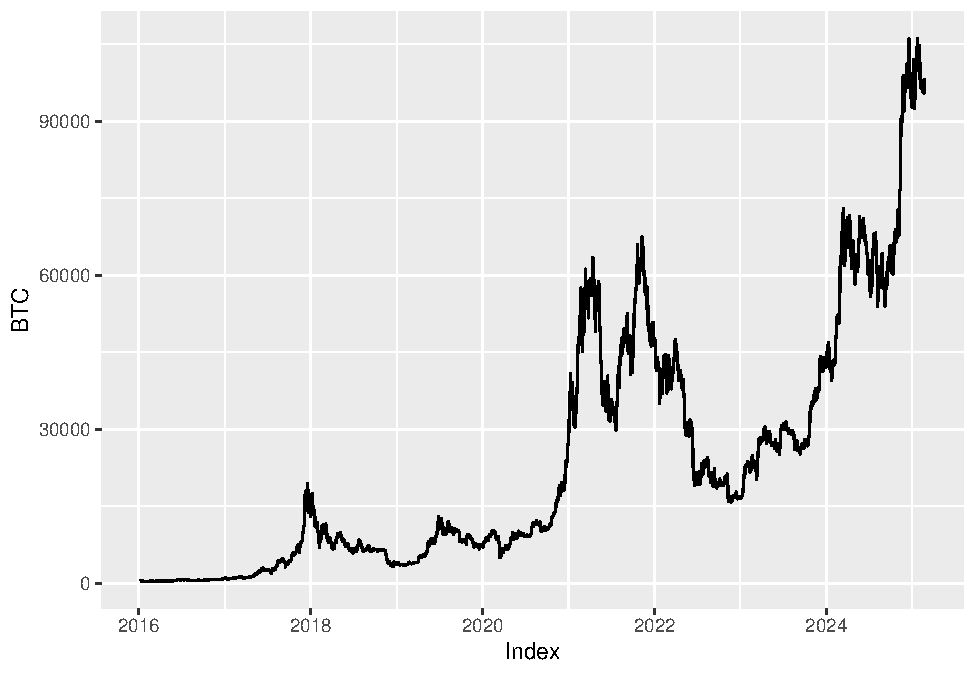
\includegraphics[width=0.85\linewidth]{Colloque_files/figure-latex/unnamed-chunk-1-1} \end{center}

\section{Introduction}\label{introduction-1}

The rapid growth of cryptocurrencies over the past decade has
transformed them into a significant component of the global financial
system. However, the volatile and non-linear nature of cryptocurrency
prices presents unique challenges for accurate forecasting. Traditional
statistical methods often fall short in capturing the intricate temporal
dependencies and high volatility of cryptocurrency time series. As a
result, researchers have increasingly turned to deep learning models,
particularly Recurrent Neural Networks (RNNs), to address these
challenges \citep{NASIRTAFRESHI2022, kumar23, seable23} .

Recurrent Neural Networks (RNNs) are well-suited for time series
forecasting due to their ability to model sequential data and capture
temporal dependencies. Variants of RNNs, such as Long Short-Term Memory
(LSTM) and Gated Recurrent Unit (GRU), have been widely adopted for
cryptocurrency forecasting. These models are particularly effective in
handling long-term dependencies and mitigating the vanishing gradient
problem, which is common in traditional RNNs. For instance,
Nasirtafreshi (2022) proposed an RNN-LSTM model to predict
cryptocurrency prices, demonstrating its ability to outperform
traditional methods in terms of accuracy.

To further enhance the predictive performance of RNNs, researchers have
explored hybrid models that combine RNNs with other techniques. For
example, Guo et al.~(2021) developed a hybrid method that integrates a
multiscale residual block with an LSTM network to forecast Bitcoin
prices. This approach leverages the strengths of both components: the
residual block captures multi-scale features, while the LSTM network
models temporal dependencies.

Similarly, other studies have proposed combining RNNs with convolutional
layers or graph-based methods to improve the model's ability to capture
spatial and temporal patterns in cryptocurrency data. The combined RNN
models offer several advantages over standalone RNNs or traditional
methods. By integrating complementary techniques, these models can
better handle the non-stationarity and noise inherent in cryptocurrency
time series. For instance, hybrid models that incorporate wavelet
transforms or attention mechanisms have been shown to improve feature
extraction and focus on relevant patterns in the data. Additionally,
ensemble approaches that aggregate predictions from multiple RNN-based
models have demonstrated enhanced robustness and accuracy in
cryptocurrency forecasting.

\section{Related works}\label{related-works}

Machine Learning is an artificial intelligence device that uses beyond
information to predict the future. In simple words, we can expect the
future price movements of cryptocurrencies to some extent by training a
machine learning model using their past price data. Some recent studies
have shown that machine learning based methods have many advantages of
using traditional forecasting models, such as the ability to produce
results that are approximately equal or identical to the actual outcome,
while also improving the precision of the outcome \citep{hitam2021}.
Decision trees, support vector machine, and neural networks are some of
the different machine learning methods that can be used for this
purpose. As evidenced by the authors in \citep{andrianto17}, the
inclusion of cryptocurrencies in multi-asset portfolios significantly
improves portfolios in several ways. To start, it will enhance the
portfolio's minimal variance and furthermore transfers the green
frontier to a higher location.

Several research studies in the literature that using machine learning
algorithms in BTC price forecasting achieve encouraging results.
According to a study \citep{hitam2021}, machine learning algorithms were
applied to perform the price prediction of many currencies including
BTC, ETH, LTC, XRP, and Stellar. According to the researchers, the SVM
model was able to beat other machine learning models in terms of
predicted values as well as accuracy. \citep{saad19} used a variety of
variables, carefully choosing the most accurate predictors using
correlation analysis. The results showed that linear regression
performed better than the other approaches when SVM, linear regression,
and random forest (RF) were used to these selected features. The authors
also tried predicting the prices of BTC and ETH using LSTM, a specific
kind of deep learning, and discovered that LSTM had the lowest
prediction error for BTC. To predict the prices of nine different
cryptocurrencies, \citep{chowdhury20} studied the application of machine
learning-based ensemble methods, namely ANN, KNN, Gradient Boosted Trees
and an ensemble model made up of multiple methods. The ensemble learning
model had the the lowest error in the predictions. \citep{derbentsev21}
studies the difficulties faced when forecasting short-term
cryptocurrency time series using supervised machine learning (ML). The
ensemble methods were then applied to the daily closing prices of
Bitcoin (BTC), Ethereum (ETH), and Ripple (XRP) using historical prices
and technical indicators such as moving averages as features: Random
Forest (RF) and Stochastic Gradient Boosting Machine (SGBM). The results
showed that ML ensemble methods held promise, with SGBM and RF yielding
good accuracy on short-term predictions.

\section*{Acknowledgement(s)}\label{acknowledgements}
\addcontentsline{toc}{section}{Acknowledgement(s)}

An unnumbered section,
e.g.~\texttt{\textbackslash{}section*\{Acknowledgements\}}, may be used
for thanks, etc.~if required and included \emph{in the non-anonymous
version} before any Notes or References.

\section*{Disclosure statement}\label{disclosure-statement}
\addcontentsline{toc}{section}{Disclosure statement}

An unnumbered section,
e.g.~\texttt{\textbackslash{}section*\{Disclosure\ statement\}}, may be
used to declare any potential conflict of interest and included \emph{in
the non-anonymous version} before any Notes or References, after any
Acknowledgements and before any Funding information.

\section*{Funding}\label{funding}
\addcontentsline{toc}{section}{Funding}

An unnumbered section,
e.g.~\texttt{\textbackslash{}section*\{Funding\}}, may be used for grant
details, etc.~if required and included \emph{in the non-anonymous
version} before any Notes or References.

\section*{Notes on contributor(s)}\label{notes-on-contributors}
\addcontentsline{toc}{section}{Notes on contributor(s)}

An unnumbered section,
e.g.~\texttt{\textbackslash{}section*\{Notes\ on\ contributors\}}, may
be included \emph{in the non-anonymous version} if required. A
photograph may be added if requested.

\section*{Nomenclature/Notation}\label{nomenclaturenotation}
\addcontentsline{toc}{section}{Nomenclature/Notation}

An unnumbered section,
e.g.~\texttt{\textbackslash{}section*\{Nomenclature\}} (or
\texttt{\textbackslash{}section*\{Notation\}}), may be included if
required, before any Notes or References.

\section*{Notes}\label{notes}
\addcontentsline{toc}{section}{Notes}

An unnumbered \texttt{Notes} section may be included before the
References (if using the \texttt{endnotes} package, use the command
\texttt{\textbackslash{}theendnotes} where the notes are to appear,
instead of creating a \texttt{\textbackslash{}section*}).

\section{References}\label{references}

\subsection{References cited in the
text}\label{references-cited-in-the-text}

\subsection{The list of references}\label{the-list-of-references}

\bibliographystyle{tfcad}
\bibliography{interactcadsample.bib}


\input{"appendix.tex"}



\end{document}
